\chapter{Libnodegit}

This section aims to give a detailed view into some important concepts and
implementation details.

\begin{figure}[htb]
  \centering
  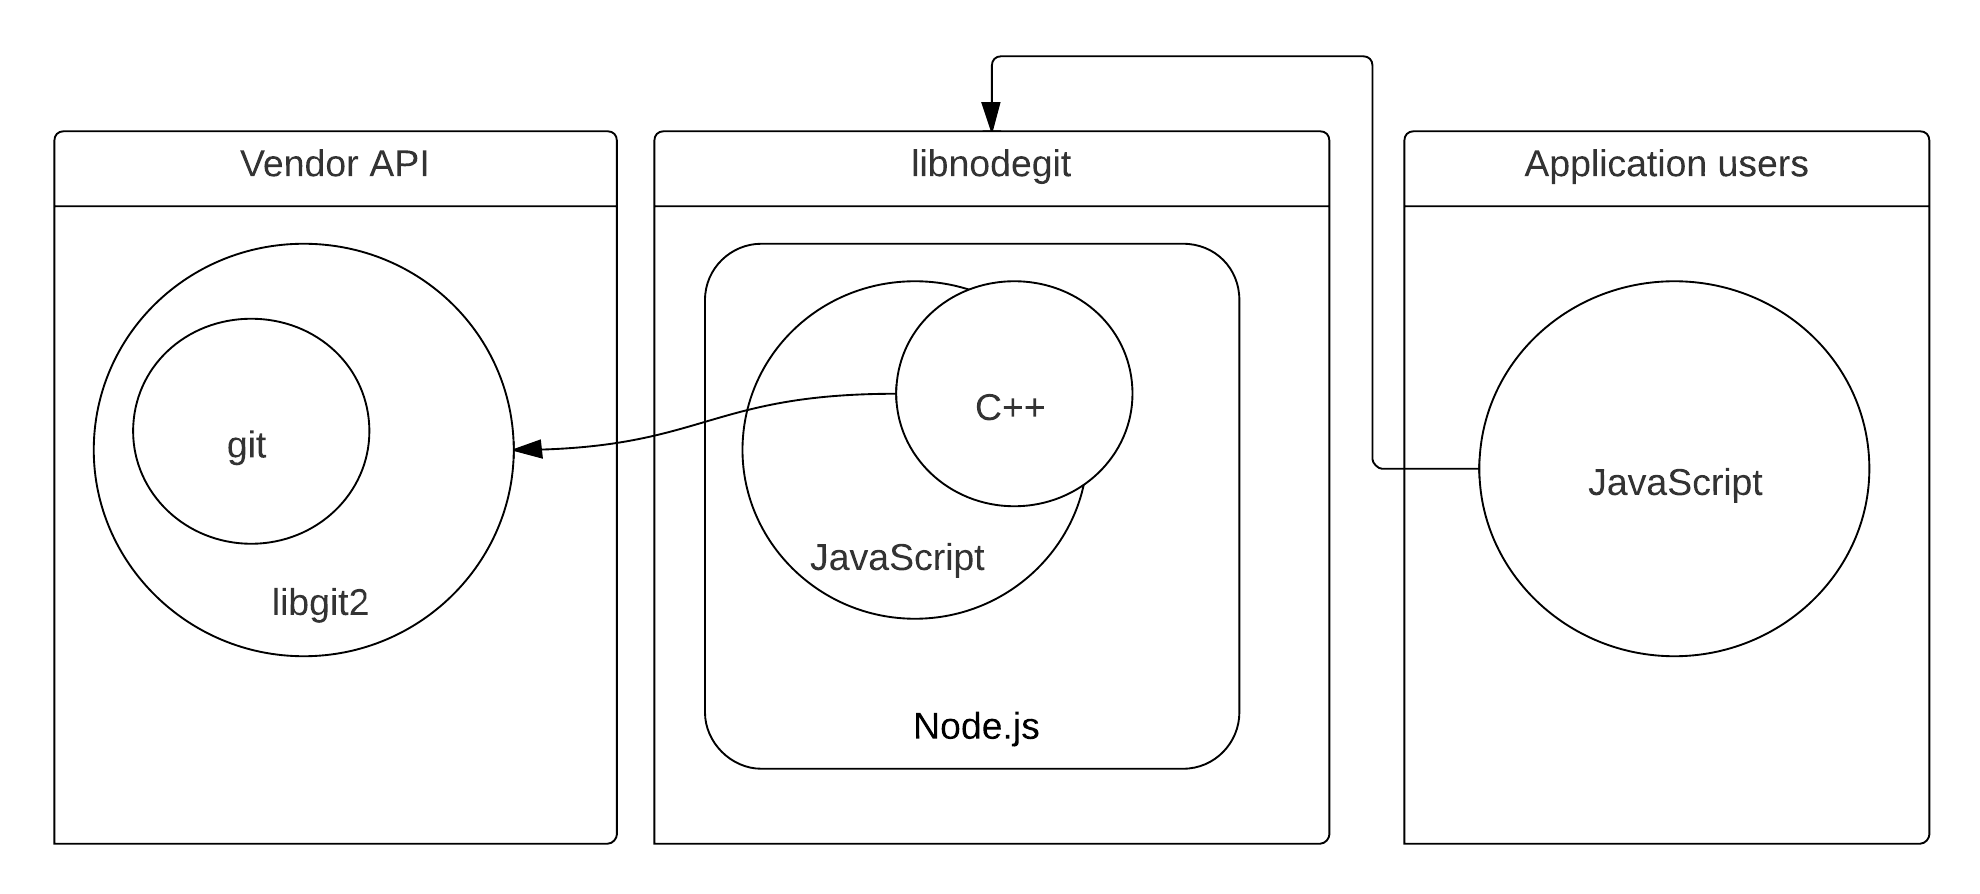
\includegraphics[scale=0.2]{./diagrams/architecture.png}
  \caption{Libnodegit architecture}
  \label{fig:architecture}
\end{figure}

\section{Design as  decisions}

\begin{description}

\item[1. Implement only the absolute minimum in C++] \hfill \\
  Jumping a level down to C++ is definitely slow for small trivial tasks. For
  eg, if function expects \texttt{n} arguments, an exception is thrown at
  JavaScript layer before dropping down to C++ if it gets less than n arguments.
  If something can be done without C++, it is ignored.

\item[2. Polish API with JS wrapper functions] \hfill \\
  Almost all functions implemented in C++, end with a trailing underscore, like
  \texttt{reference\_} and is never exposed from the API. An equivalent wrapper
  function in JavaScript will be called \texttt{reference}, which will make sure
  that the arguments are correct, call the underlying C++ implementation and
  returns the result with appropriate modifications.

\item[3. Prefer lazy evaluation wherever possible] \hfill \\
  Wrapper functions are used for lazy evaluation for performance. For example,
  the C++ function \texttt{parents\_} return an array of SHA1 strings, and the
  wrapper function \textit{parents} converts it into an array of reference
  instances only when the function is explicitly called.

\item[4. Automate tasks with Makefiles and build tools like gyp] \hfill \\
\item[5. Write tests to ensure correctness wherever possible] \hfill \\

\end{description}

\section{API}

The API is essentially is an abstraction from the low level \texttt{git
  --plumping} or \texttt{libgit2} to a higher level. It is explained with
examples.

\subsection{API example - \texttt{git log}}

The simplest of the git operations is to see the log of the project history.
Here is an example of getting the details of the last 3 commits from the
libnodegit project the normal git way.

\begin{verbatim}

$ cd Projects/libnodegit/
$ git log -3

commit 1a9973aacc3a080add250228a9cee571945e72ec
Author: Jaseem Abid <jaseemabid@gmail.com>
Date:   Fri Apr 26 19:23:21 2013 +0530

    README fixes

commit 0dd1b45b20a1e4827d268f1b859ffcb5dd39069d
Author: Jaseem Abid <jaseemabid@gmail.com>
Date:   Sat Apr 20 07:37:04 2013 +0530

    `npm link` loops calling npm rebuild

    This might be the issue, deal later.
    https://github.com/isaacs/npm/issues/2788

commit 01b58820ae28938dec9bb5575afc4624a992b21d
Author: Jaseem Abid <jaseemabid@gmail.com>
Date:   Mon Mar 25 21:15:30 2013 +0530

    Whitespace fixes

\end{verbatim}

Its quite easy and convenient for humans to parse this output and get the
required information out of it. Consider parsing this for machine consumption.
Getting a list of SHA1 ids or emails out of this takes us back to regular
expressions and language parsers - an overhead and error prone task. This is
what libnodegit is trying to improve.

Here is the same task with libnodegit library.

\begin{verbatim}

# Require the library
l = require "libnodegit"

# Initialize the repo with path alone
repo = new l.Repository "~/Projects/libnodegit"

# Get last 2 commits
commits = repo.log {count : 2}

# Print the commits array
console.log commits

// Commits array
[
    {
      "commit": "1a9973aacc3a080add250228a9cee571945e72ec",
      "author": {
        "name": "Jaseem Abid",
        "email": "jaseemabid@gmail.com"
      },
      "date": "Fri Apr 26 19:23:21 2013 +0530",
      "message": "README fixes"
    },
    {
      "commit": "0dd1b45b20a1e4827d268f1b859ffcb5dd39069d",
      "author ": {
        "name": "Jaseem Abid",
        "email": "jaseemabid@gmail.com>"
      },
      "date": "Sat Apr 20 07:37:04 2013 +0530",
      "message": "`npm link` loops calling npm rebuild''
    }
]

\end{verbatim}

In the example, the log function returns an array of commit objects, each with
its own properties which can be easily manipulated and required information can
be easily filtered from it. Extracting the list of SHA ids is a trivial task
here.
